% Fig 3.15 ESR with S=1: (a) Zeeman levels E = g mu_B B m (m=1,0,-1) and single-line
% absorption; (b) with axial crystal-field shift -Delta of m=0 level and double-line
% absorption. 2x2 layout: (a) levels | (a) spectrum // (b) levels | (b) spectrum.
\documentclass[tikz,border=5pt]{standalone}
\usetikzlibrary{arrows.meta}
\usepackage{amsmath}
\usepackage{bm}
\usepackage{fontspec}
\setmainfont{Times New Roman}
\begin{document}
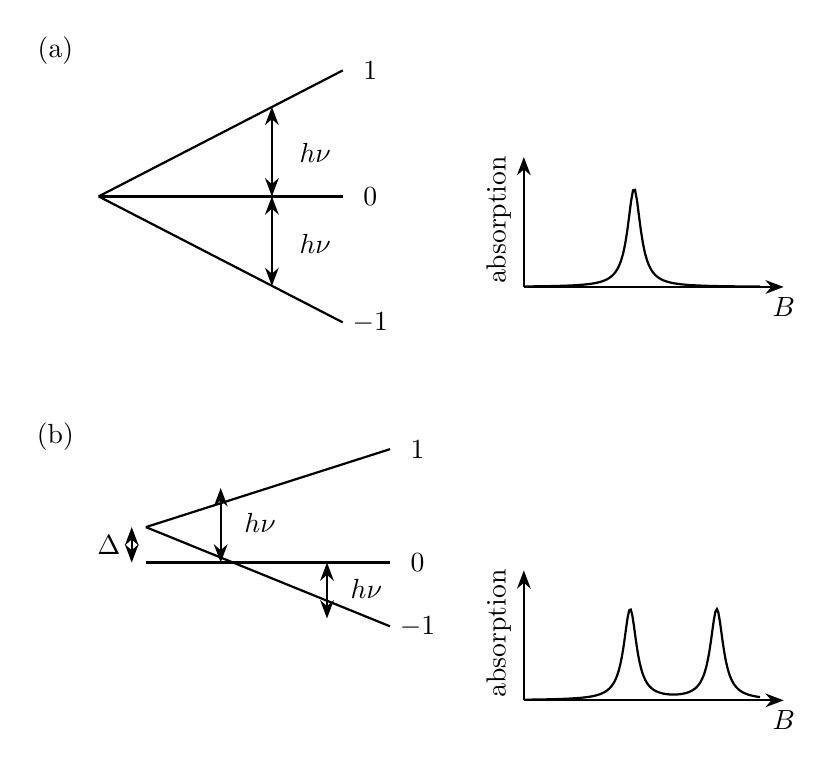
\begin{tikzpicture}[line width=0.8pt,>=Stealth]
% ================= row (a) =================
\begin{scope}[shift={(0,0)}]
\node at (-0.55,3.35) {(a)};
% levels: fan from apex, slopes +, 0, -
\draw[thick] (0,1.5) -- (3.1,3.10);
\draw[thick] (0,1.5) -- (3.1,1.50);
\draw[thick] (0,1.5) -- (3.1,-0.10);
\node at (3.45,3.10) {$1$};
\node at (3.45,1.50) {$0$};
\node at (3.45,-0.10) {$-1$};
% h nu double arrows between adjacent levels
\draw[<->] (2.2,2.638) -- (2.2,1.5);
\draw[<->] (2.2,1.5) -- (2.2,0.362);
\node at (2.75,2.05) {$h\nu$};
\node at (2.75,0.90) {$h\nu$};
% spectrum: single Lorentzian
\begin{scope}[shift={(5.4,0.35)}]
  \draw[->] (0,0) -- (3.3,0) node[below] {$B$};
  \draw[->] (0,0) -- (0,1.65);
  \node[rotate=90] at (-0.32,0.85) {absorption};
  \draw[thick] plot[domain=0:3.0,samples=120]
    ({\x},{1.25/(1+((\x-1.4)/0.10)^2)});
\end{scope}
\end{scope}
% ================= row (b) =================
\begin{scope}[shift={(0,-4.9)}]
\node at (-0.55,3.35) {(b)};
% levels: apex for m=+/-1, m=0 line shifted down by Delta
\draw[thick] (0.6,2.2) -- (3.7,3.19);
\draw[thick] (0.6,1.75) -- (3.7,1.75);
\draw[thick] (0.6,2.2) -- (3.7,0.94);
\node at (4.05,3.19) {$1$};
\node at (4.05,1.75) {$0$};
\node at (4.05,0.94) {$-1$};
% Delta shift at B=0
\draw[<->] (0.42,2.2) -- (0.42,1.75);
\node at (0.13,1.97) {$\Delta$};
% h nu arrows: 1<->0 at small B, 0<->-1 at larger B
\draw[<->] (1.55,2.696) -- (1.55,1.75);
\node at (2.05,2.25) {$h\nu$};
\draw[<->] (2.9,1.75) -- (2.9,1.04);
\node at (3.4,1.42) {$h\nu$};
% spectrum: two Lorentzians
\begin{scope}[shift={(5.4,0.0)}]
  \draw[->] (0,0) -- (3.3,0) node[below] {$B$};
  \draw[->] (0,0) -- (0,1.65);
  \node[rotate=90] at (-0.32,0.85) {absorption};
  \draw[thick] plot[domain=0:3.0,samples=160]
    ({\x},{1.15/(1+((\x-1.35)/0.10)^2)+1.15/(1+((\x-2.45)/0.10)^2)});
\end{scope}
\end{scope}
\end{tikzpicture}
\end{document}
